% Active lag circuit: the scanned schematic (active_lag.png) with the signal
% labels drawn over it in red. Build with `make figures/active_lag.pdf`.
%
% Coordinates are in the scan's own pixels, origin top left, y pointing down,
% so a label is moved by nudging the numbers.
\documentclass[border=0pt]{standalone}
\usepackage{tikz}
\usetikzlibrary{arrows.meta}

\begin{document}
\begin{tikzpicture}[x=0.01cm, y=-0.01cm,
    lbl/.style={red, font=\small},
    flow/.style={red, thick, -{Stealth[length=5pt]}}]
  \useasboundingbox (0,0) rectangle (690,251);
  \node[anchor=north west, inner sep=0] at (0,0)
    {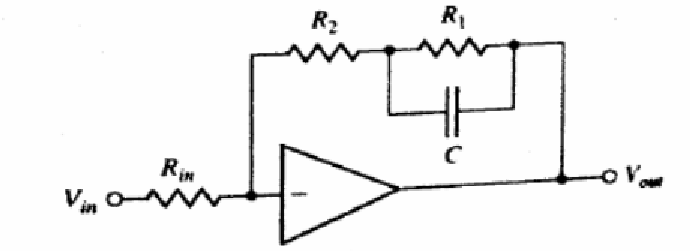
\includegraphics[width=6.9cm]{active_lag.png}};

  % currents
  \draw[flow] (222,197) -- (246,197) node[lbl, midway, above=1pt] {$i_{in}$};
  \draw[flow] (256,53)  -- (282,53)  node[lbl, midway, above=1pt] {$i_{in}$};
  \draw[flow] (488,44)  -- (510,44)  node[lbl, midway, above=1pt] {$i_1$};
  \draw[flow] (398,109) -- (432,109) node[lbl, midway, below=1pt] {$i_c$};

  % voltages, + on the end the current enters
  \node[lbl] at (283,80) {$+$};  \node[lbl] at (322,84) {$V_2$};  \node[lbl] at (362,80) {$-$};
  \node[lbl] at (405,72) {$+$};  \node[lbl] at (452,74) {$V_1$};  \node[lbl] at (500,72) {$-$};
\end{tikzpicture}
\end{document}
